\documentclass[border=4pt]{standalone}
\usepackage{amsmath,amssymb,bm,mathtools}
\usepackage{tikz}
\usetikzlibrary{positioning,calc,arrows.meta}
\usepackage{xcolor}
\definecolor{blue}{HTML}{1F618D}\definecolor{red}{HTML}{B03A2E}\definecolor{gray}{HTML}{7F7F7F}
\definecolor{ink}{HTML}{111111}
% Geometry: three tiers of width W, centred on x = W/2; halves of width W/2
\newcommand{\W}{11.2}      % total width (cm)
\newcommand{\C}{5.6}       % centre x = W/2
\newcommand{\Lc}{2.8}      % centre of left half  = W/4
\newcommand{\Rc}{8.4}      % centre of right half = 3W/4
\begin{document}
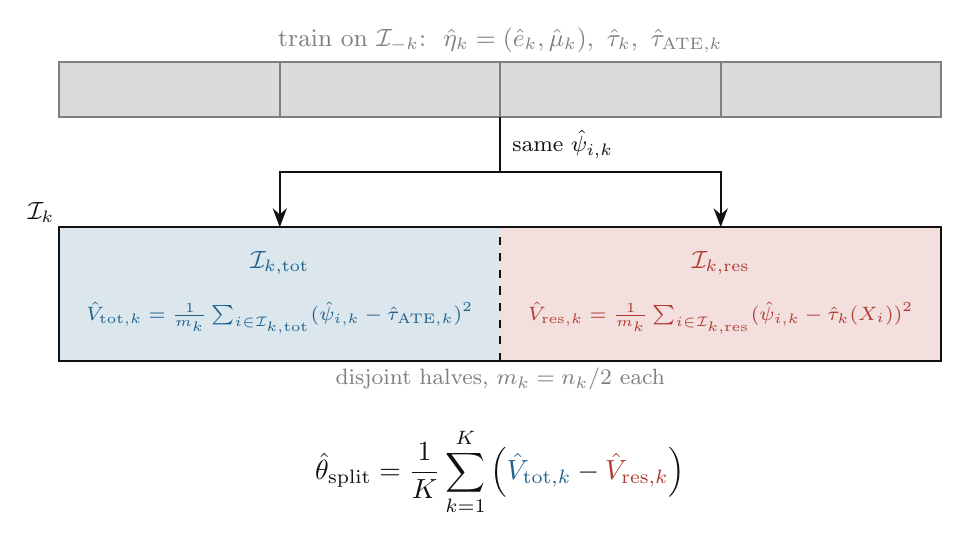
\begin{tikzpicture}[x=1cm,y=1cm, every node/.style={text=ink}, line width=0.7pt, >={Stealth[length=2.4mm]}]
% ---- TIER A: out-of-fold training data I_{-k}: grey strip of four equal cells (the K-1 training folds)
\fill[gray!28] (0,0) rectangle (\W,0.7);
\draw[gray] (0,0) rectangle (\W,0.7);
\foreach \i in {1,2,3} { \draw[gray] (\i*\W/4,0) -- (\i*\W/4,0.7); }
\node[above=3pt, font=\small, text=gray, inner sep=0pt] at (\C,0.7)
  {train on $\mathcal{I}_{-k}$:\ \ $\hat\eta_k=(\hat e_k,\hat\mu_k),\ \hat\tau_k,\ \hat\tau_{\mathrm{ATE},k}$};
% ---- TIER B: evaluation fold I_k, randomly bisected into two equal disjoint halves
\fill[blue!16] (0,-3.1) rectangle (\C,-1.4);
\fill[red!16]  (\C,-3.1) rectangle (\W,-1.4);
\draw[ink] (0,-3.1) rectangle (\W,-1.4);
\draw[ink, dashed] (\C,-3.1) -- (\C,-1.4);
\node[font=\small, text=blue, inner sep=0pt] at (\Lc,-1.85) {$\mathcal{I}_{k,\mathrm{tot}}$};
\node[font=\small, text=red,  inner sep=0pt] at (\Rc,-1.85) {$\mathcal{I}_{k,\mathrm{res}}$};
\node[font=\scriptsize, text=blue, inner sep=0pt] at (\Lc,-2.55)
  {$\hat V_{\mathrm{tot},k}=\frac{1}{m_k}\sum_{i\in\mathcal{I}_{k,\mathrm{tot}}}(\hat\psi_{i,k}-\hat\tau_{\mathrm{ATE},k})^2$};
\node[font=\scriptsize, text=red,  inner sep=0pt] at (\Rc,-2.55)
  {$\hat V_{\mathrm{res},k}=\frac{1}{m_k}\sum_{i\in\mathcal{I}_{k,\mathrm{res}}}(\hat\psi_{i,k}-\hat\tau_k(X_i))^2$};
\node[font=\small, inner sep=0pt, anchor=south east] at (-0.05,-1.35) {$\mathcal{I}_k$};
\node[below=2pt, font=\footnotesize, text=gray, inner sep=0pt] at (\C,-3.1) {disjoint halves, $m_k=n_k/2$ each};
% ---- CONNECTOR: one stem forking into two heads -- the identical nuisances feed both halves
\draw[ink, ->] (\C,0) -- (\C,-0.7) -| (\Lc,-1.4);
\draw[ink, ->] (\C,-0.7) -| (\Rc,-1.4);
\node[font=\footnotesize, right=4pt, inner sep=0pt] at (\C,-0.35) {same $\hat\psi_{i,k}$};
% ---- TIER C: aggregation across folds
\node[anchor=north, inner sep=0pt] at (\C,-3.95)
  {$\displaystyle \hat\theta_{\mathrm{split}}=\frac{1}{K}\sum_{k=1}^{K}\Big(\textcolor{blue}{\hat V_{\mathrm{tot},k}}-\textcolor{red}{\hat V_{\mathrm{res},k}}\Big)$};
\end{tikzpicture}
\end{document}
